\section{Results}

Implementation of the proximal Newton method is provided in the \texttt{R} package \href{https://dajmcdon.github.io/rtestim/}{\texttt{rtestim}}. 

\subsection{Covid-19 cases}

% introduce data & hyperparameter setup
We implement the proposed model on the Covid-19 confirmed cases in British Columbia (B.C.) as of May 18, 2023 reported by B.C. Conservation Data Centre. We choose the gamma distribution with shape $2.5$ and scale $2.5$ to approximate the serial interval function.

%\begin{figure}[tb]
%    \centering
    %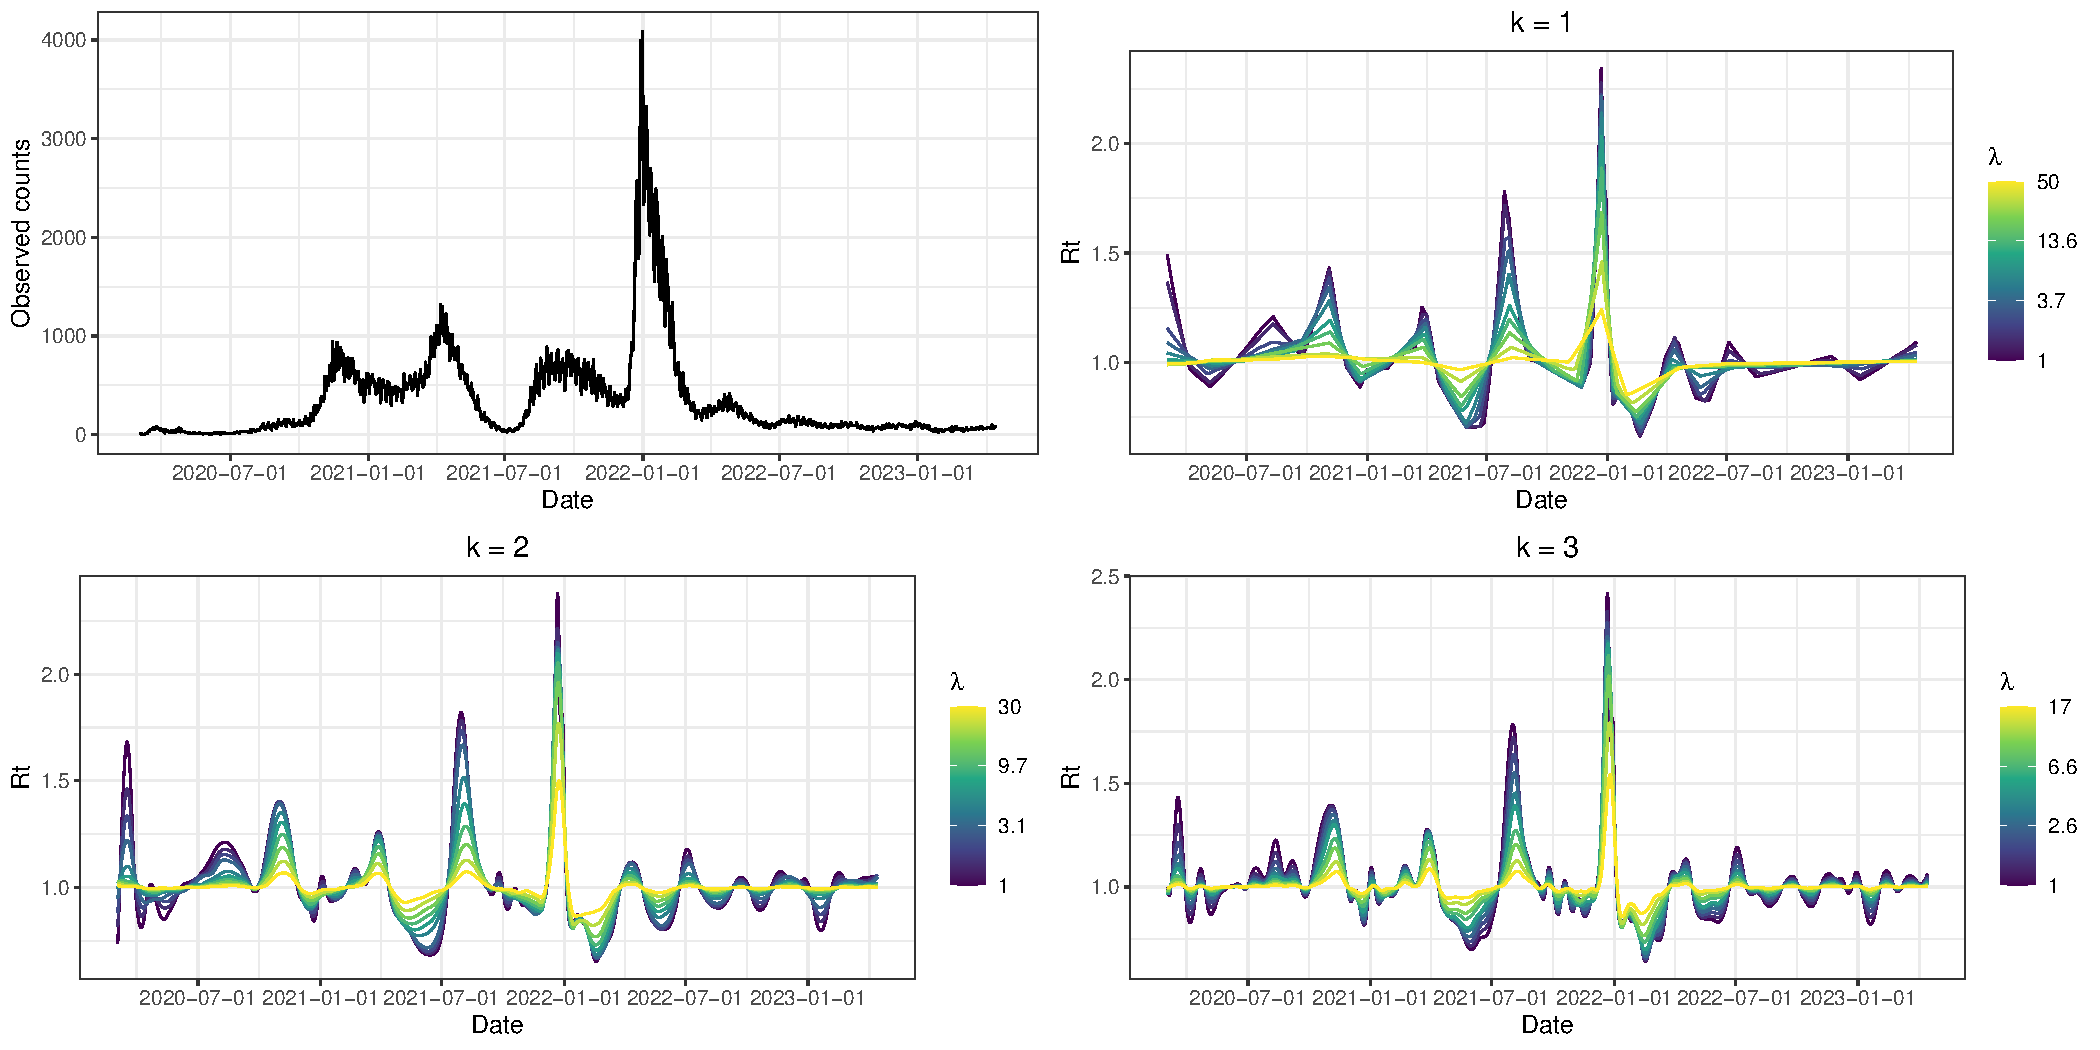
\includegraphics[width=0.99\linewidth]{fig/covid19fig.pdf}
%    \caption{Covid19 daily confirmed counts between March 1st, 2020 and April 15th, 2023 in British Columbia, Canada. The top left panel displays the time trend of the observed infectious cases. The top right, bottom left and bottom right panels illustrated the estimated reproduction numbers ($\calR_t$) using the Poisson trend filtering (in \eqref{eq:rt-ptf}) with degrees $k=1,2,3$ respectively.} 
%\end{figure} 

% interpret figures -- across all lambdas
Considering the temporal evolutions of neighboring $3, 4, 5$ reproduction numbers, the estimated reproduction numbers of Covid-19 in British Columbia (displayed in the top right, bottom left, and bottom right panels in Fig 1 respectively) are always lower than $2.5$, which means that two distinct infected individuals can on average infect less than five other individuals in the population. The three degrees of the temporal evolution (across all regularization levels $\lambda$) all yield similar results that $\hat{\calR}_t$ achieves the highest peak around the end of 2021 and reaches the lowest trough shortly thereafter. Throughout the estimated curves, the peaks and troughs of the reproduction numbers roughly come prior to the following growths and decays of confirmed cases respectively.

The reproduction numbers are relatively unstable before April 1st, 2022.
The highest peak coincides with the emergence and globally spread of the Omicron variant. The estimated reproduction numbers are apparently below the threshold $1$ during two time periods -- roughly from April 1st, 2021 to July 1st, 2021 and from January 1st, 2022 to April 1st, 2022. The first trough of $\hat{\calR}_t$ coincides with the first authorization for use of Covid-19 vaccines in British Columbia. The second trough shortly after the greatest peak may credit to many aspects, including self-isolation of the infected individuals and application of the second shot of Covid-19 vaccines. 
Since around April 1st, 2022, the reproduction numbers stay stable (at around $1$) and the infected cases stay low. 

% for different lambda
Greater regularization levels (i.e., larger $\lambda$s) result in smoother estimated curves. Smoother curves (e.g., the yellow curve in the top right panel in Fig 1) suggest that the estimated reproduction numbers are around $1$ during most time periods; however, they may not be appropriate to interpret the reality. More wiggly curves better reflect the fluctuation of $\calR_t$, but sometimes fail to highlight the significant peaks or troughs. The tuning parameter $\lambda$ needs to be chosen corresponding to the information in practice for a better interpretation.
